\section{System Architecture and Goals}
The subsequent sections overview the SampleClean projects, and this section describes some of the general principles, challenges, and design goals. 

\subsection{Architecture}
At a high-level all SampleClean projects apply a user-specified data transformation to a maximum of $k$ out of $N$ rows in a relation, and estimate the \emph{true} result, i.e., if all the data were transformed, of some data analytics. Figure \ref{fig:arch} describes the basic architecture of these problems. 

\vspace{0.5em}
\noindent\textbf{Initialization: } The system is initialized with a dirty relation $R$, a user specified data cleaning technique $C(\cdot)$, a budget $k$, and some analytic query to run $q$. SampleClean provides a framework to execute the cleaner no more than $k$ times and estimate the result of $q$.  

\vspace{0.5em}
\noindent\textbf{Analytics: } In the basic problem setting, the supported queries are aggregates of the form:
\begin{alltt}
q = SELECT \textsf{f}(attrs) FROM R WHERE predicate GROUP BY attrs
\end{alltt}
In \sampleclean, we consider \avgfunc, \sumfunc, \countfunc, and \varfunc.
In View Cleaning, we extend this set of queries to any queries whose confidence intervals can be estimated with a statistical bootstrap \cite{agarwalknowing}. 
Finally, in ActiveClean, we extend this work to consider Machine Learning models as aggregate queries.

\vspace{0.5em}
\noindent\textbf{Sampler: } The first component of SampleClean is the sampler. The sampler selects a sample of $k$ rows from the dirty relation $R$. For each sampled row $i$, the sampler maintains a sampling probability $p_i$. The sampler is one of the primary points for optimization in this project. In SampleClean, we used a uniform sample of $k$ rows from $R$.
In View Cleaning, we select a uniform sample of $k$ rows from a view $R$, where there is some known view definition.
And in ActiveClean, we use the analytic query $q$ to select a non-uniform sample of rows from $R$.

\vspace{0.5em}
\noindent\textbf{Cleaner: }
Given the sample of dirty rows $S_{dirty}$,  the cleaner applies the user-specified data cleaning $C(\cdot)$. There are two data cleaning models for $C(\cdot)$: \emph{row-by-row} and \emph{set-of-rows}.
Formally, a row-by-row cleaner is applied to every row in $S_{dirty}$ and possibly changes the sampling probability as well (e.g., deduplication):
\[
(S_{clean},p_i') = \{C(r) : \forall (r,p_i) \in (S_{dirty},p_i)\}
\]
This model captures common blocking-matching entity resolution and deduplication, extraction, filtering, and value filling.

The row-by-row cleaning model is a formalization of the costs of data cleaning where each row has the same cost to clean and this cost does not change throughout the entire cleaning session.
There are, however, some cases when cleaning the first row of a certain type of corruption is expensive but all subsequent row are cheaper.
Consider a spell checker that allows the user to fix all similarly misspelled words. 

To address this problem, we also study the set-of-rows cleaning model.
In the set-of-rows model, the cleaning function $C(\cdot)$ is not restricted to updating only the rows in the sample.
$C(\cdot)$ takes the entire dirty sample as an argument (that is the cleaning is a function of the sample), the dirty data, and updates the entire dirty data:
\[
(S_{clean}, R'_{dirty}) = C(S_{dirty},R_{dirty})
\]
we require that for every record $s \in S_{dirty}$, that record is completely cleaned after applying $C(\cdot)$, giving us $S_{clean}$.

\vspace{0.5em}
\noindent\textbf{Estimator: } The goal of the estimator is to estimate the value of $q(R_{clean})$ from the cleaned sample $S_{clean}$, the dirty sample $S_{dirty}$, and the sampling probabilities $p_i'$. The estimator possibly has to modify $q$ to account for scaling differences when running the query on the sample.

\begin{SCfigure}
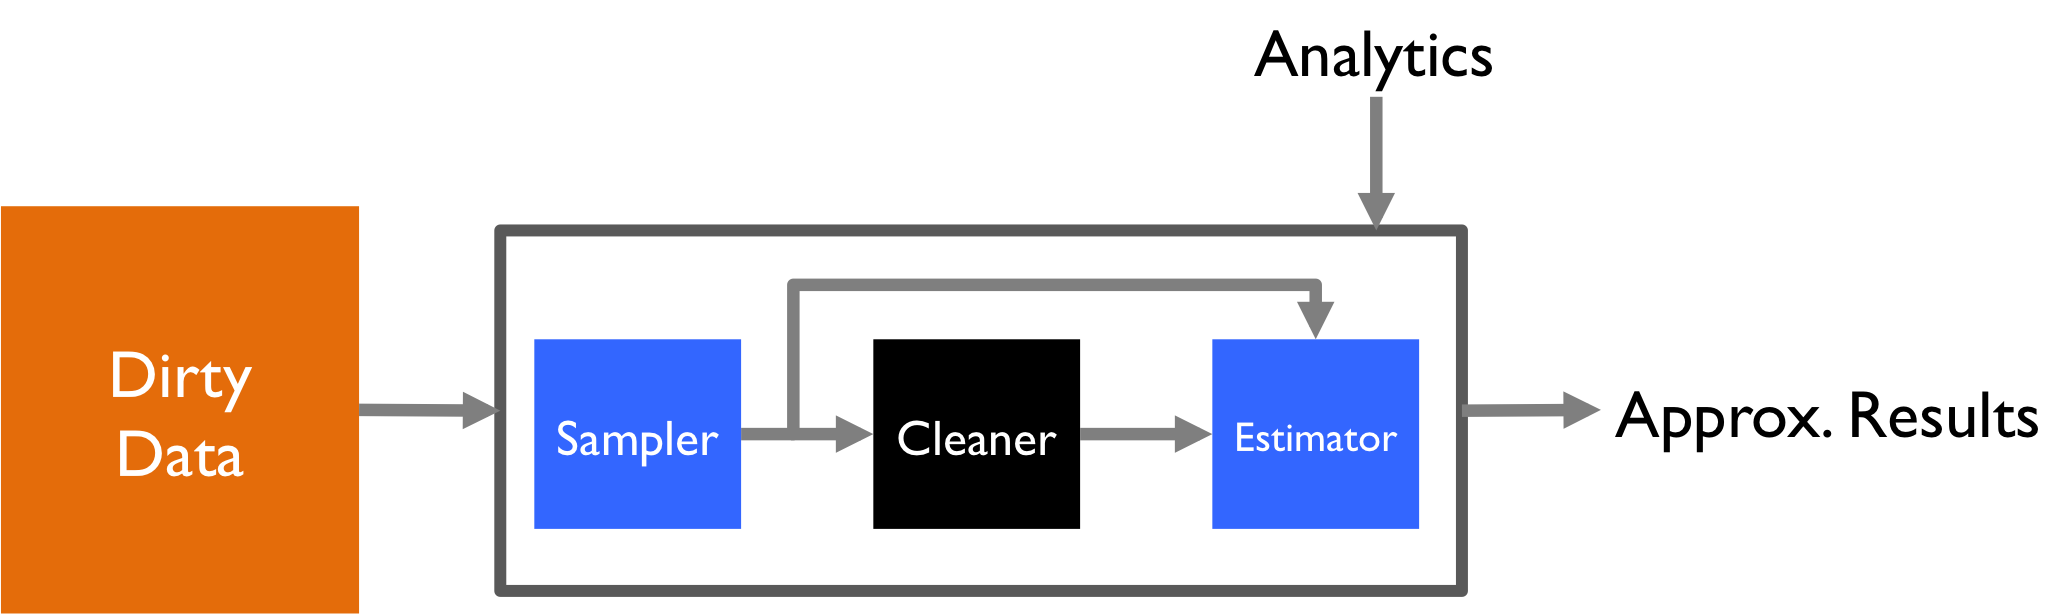
\includegraphics[width=.5\columnwidth]{figs/arch.png}
\caption{Given a user-specified data cleaning operation, SampleClean applies this operation to a sample, and estimates the result of data analytics. \label{fig:arch}}
\end{SCfigure}

\subsection{Methogology Matters}
From interviews with data scientists in technology companies, we found that many already sample data when prototyping expensive data transformations.
The contribution of SampleClean is to recognize that certain methodologies for sampling and cleaning can lead to inaccurate or even misleading results.
SampleClean provides a framework to apply budgeted data cleaning in a reliable way with provable guarantees on the result.

\vspace{0.5em}
\noindent\textbf{Not Only About Latency: } As applied in SampleClean, random sampling is not only a technique to reduce the latency of data cleaning but also a technique to simultaneously estimate the impact of data error.
When errors are unknown and systematic, the randomization of sampling allows us to bound the estimates.
One of the goals of this project is to develop reliable estimation techniques that will work in a wide variety of error and query regimes.

\vspace{0.5em}
\noindent\textbf{Unbiasedness: } For some types of analytics, we can guarantee that the estimate is unbiased. This means that, in expectation, over all samples of size $k$ the estimate is equal to the true value. Unbiased estimates are useful since a confidence interval measuring the precision of the estimate is equivalent to measuring accuracy w.r.t to the fully cleaned result.

\vspace{0.5em}
\noindent\textbf{Confidence Intervals: } SampleClean bounds every estimate in a confidence interval. This is a significant result since, without data cleaning, the error is potentially unbounded. Bounded estimates (even if loose) give the analyst guidance on how inaccurate an estimate is.

\subsection{Wisteria: Implementing SampleClean \cite{haas2015wisteria}}
The ideas in SampleClean are implemented as a part of a distributed data cleaning library named Wisteria (Figure \ref{fig:ex-plan}).
Wisteria is built on the Berkeley Data Analytics Stack with numerous optimized data cleaning primitives.
This insight of this project was that the data cleaning process is inherently iterative, with evolving cleaning workflows that 
start with basic exploratory data analysis on small samples of dirty data, then refine analysis with 
more sophisticated/expensive cleaning operators (e.g., crowdsourcing), and finally apply the insights to a full dataset.
Wisteria designed to support the iterative development and optimization of data cleaning workflows, especially ones that utilize the crowd.

In Wisteria, sampling is a first-class logical operator for data cleaning plans that tolerate approximation, and use it to speed up iteration on early-stage plans.
Analysts can prototype expensive data cleaning operations and estimate the effects using samples.
The samples also serve to tune data cleaning plans and a recommendation engine proposes changes to in-flight cleaning plans that allow users to trade off accuracy and latency, and the system provides efficient mechanisms for implementing recommended changes without re-executing the plan on already cleaned tuples.

\begin{SCfigure}
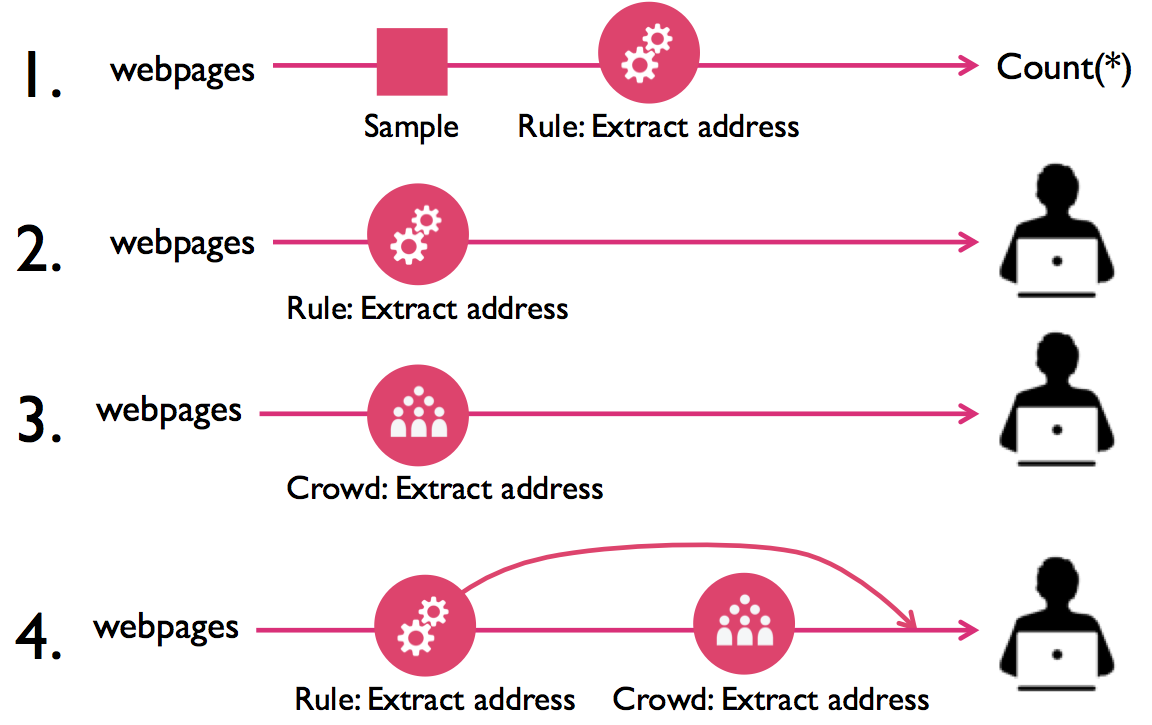
\includegraphics[width = .4\textwidth]{figs/lifecycle.png}
\caption{
1) The analyst starts with an exploratory plan that uses a sample to evaluate a simple address extraction method.
2) A plan that applies the method to the entire dataset. The quality is unsatisfactory. 
3) An alternate plan that uses manual crowd extraction. The quality is now high, but the crowd-based extractor is slow. 
4) A hybrid plan that sends only difficult webpages to the crowd, maximizing accuracy without sacrificing latency.}
\label{fig:ex-plan}
\end{SCfigure}



